\section{Experiment protocol for test subjects} \label{sec:protocol:experiment}

\textbf{Title of the project} \\
Using confidence levels of movement recognition in user training to improve prosthesis control 

\textbf{Details on investigators} \\
All investigators are 2nd semester biomedical engineering master students at Aalborg University.  

\textbf{Purpose} \\
The purpose of this experiment is to train the subject in getting better at controlling a functional prosthesis. The subject will be training seven hand movements that is used in activating the prosthesis. In the experiment the prosthesis will be represented on a computer screen, where the subject will receive visual feedback on how the prosthesis interpret the hand movement performed by the subject. By receiving this visual feedback it is hypothesized that the user will get better at controlling the prosthesis over time. 

\textbf{Background} \\
Electromyography (EMG), or muscle signals, is widely used for controlling functional lower arm prosthetics for transradial amputees. The ideal purpose of a functional prosthesis is to behave as functional as possible compared to a biological arm. Functional prosthetics that rely on pattern recognition-based control are becoming exceedingly good in performance in a clinical environment, due to highly optimized system control. However, still only one commercially available pattern recognition-based prosthesis exist. Users reject these functional prosthetics usually due to functionality issues when utilizing them in daily life tasks outside the clinical environment. Many improvements have been made in the area of system control, but another approach of improving the prosthetic control is by training the user. User training has only been explored scarcely in the research literature, thus, new techniques to improve the user's ability to control a prosthesis are yet untouched. This experiment will focus on training the user to improve prosthetic control on a fixed pattern recognition-based control system. The novel approach in this study is to provide the user with information on how well the system recognizes the performed movement during user training. 

%Commercially available prosthesis have yet to adopt the use of pattern recognition methods in their control scheme. Mainly, this is due to the disadvantages exploited in “ref til introduction om problemer måske?”. A control scheme that reduce these disadvantages are therefore sought through the combination of regression and classification based methods. 
%The overall aim is to develop a novel control scheme for myoelectric prosthetic devices. Hereby it is sought to clarify if a combined regression and classification control scheme yields higher subject performance in a Fitts’ Law test compared to a method only using regression.

\textbf{Research hypothesis} \\
Exposing subjects to user training, in which confidence levels of movement recognition is used as feedback, will show statistically significant improvement in performance in a classification-based myoelectric prosthetic control scheme, when compared to subjects who have not had the same feedback during user training.% across short training sessions. 

%\textbf{Ethical considerations}  \\
%The investigators do not foresee any obstacles of ethical nature during the proceedings of this experiment. No test subjects will be exposed to any physical interventions besides being asked to wear the Myo armband. We expect that no part of this experiment puts the subject in any danger. 

\textbf{Session time} \\
The experiment consist of three sessions, which are spread over three consecutive days; one session per day. Each session is estimated to have a total duration of 30-60 minutes. 

\textbf{Inclusion criteria} \\
The subject needs to be:
\begin{itemize}
	\item able bodied.
	\item above 18 years old.
	\item able to read, understand and speak Danish and/or English.
	\item assessed by the investigators to understand and perform the instructions given during the experiment. 
\end{itemize}


\textbf{Exclusion criteria} \\
The subject must not have:
\begin{itemize}
	\item diseases that might influence subject performance. 
\end{itemize}


\textbf{\Large{Experiment procedure}}

The experiment consists of three sessions containing different procedures as illustrated on \figref{fig:experiment_protocol_pipeline}. The concept and chronology of each procedure is described below the illustration. During the experiment it is important that the subject is placed sitting on a chair, with the arm wearing the Myo armband (MYB) hanging relaxed down by the side of the body, as shown in \figref{fig:experiment_setup} on page \pageref{fig:experiment_setup} illustrating the experiment setup. 

\begin{figure}[H]                                         
	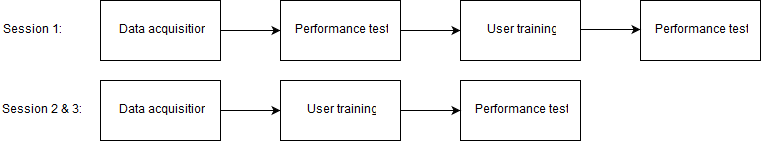
\includegraphics[width=0.9\textwidth]{figures/pMethods/experiment_protocol_pipeline}  
	\caption{Pipeline for the three sessions in the experiment and what procedures each session contains.}
	\label{fig:experiment_protocol_pipeline} 
\end{figure}


\textbf{Data acquisition} \\
For the myoelectric control system to be able to identify a performed movement as the movement that is actually performed, it needs information about how the movement looks when represented as a EMG signal. Thus, EMG data needs to be acquired from the forearm of the subject while the subject performs the movements that is used in the experiment, see \figref{fig:experiment_movements} on page \pageref{fig:experiment_movements}. This data is fed to the control system to train the system to recognize each movement. In this experiment EMG data will be acquired from the subject with an EMG-electrode armband: MYB from Thalmic Labs. The chronology of this procedure is as follows:

\begin{enumerate}
	\item Apply MYB on dominant forearm at the thickest part.
	\item Synchronize MYB by performing wrist extension until three distinct vibrations are felt from the MYB.
	\item Perform 15 seconds of maximum voluntary contraction (MVC) of instructed movement. The MVC is a contraction the subject is able to withhold in a constant intensity for the 15 seconds. Following the MVC the subject will be given a 30 seconds resting period to avoid muscle fatigue.
	\item Perform three 15 seconds contraction trails of respectively 40\%, 50\% and 70\% of MVC. During these contractions the subject will control a green marker representing the EMG signal and try to follow a trapezoidal trajectory as precise as possible. The trapezoidal trajectory consists of two 2.5 second transition phases and one 5 second plateau phase. Between each trial the subject will be given a 10 seconds resting period to avoid muscle fatigue.
	\item Repeat step 3-4 until training data from all four wrist movements has been recorded.
\end{enumerate}

An illustration of the interface used for data acquisition is shown in \figref{fig:dataacqGUI}.

\begin{figure}[H]                 
	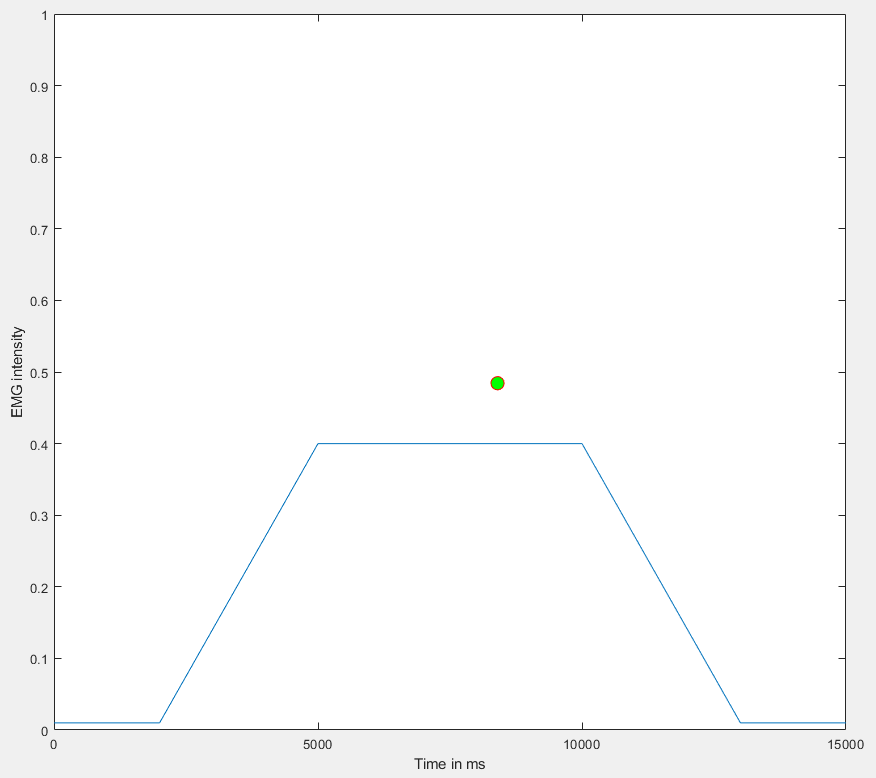
\includegraphics[width=.8\textwidth]{figures/xBackground/dataacqGUI2}  
	\caption{Illustration of the data acquisition interface showing the trapezoidal trajectory and the green marker representing the EMG signal.}
	\label{fig:dataacqGUI} 
\end{figure}

\textbf{User training} \\ %test group
The purpose of user training is for the subject to train the movements used in the performance test. During the user training the subject will train one movement at a time at different contraction levels. When training a movement, visual feedback in form of confidence levels on how well the control system recognizes movements, is shown in percentage in a bar plot. In addition, the level of contraction is shown in a horizontal bar above the other bar plot. When performing the instructed movement at the instructed level of contraction the horizontal bar plot will appear green; if it is outside the instructed level or if the system does not recognize the performed movement, it appears red. The aim for the subject is to reach and withhold the instructed contraction level with 100 \% confidence for each movement. When the subject withholds the contraction level inside the instructed contraction level for 1 seconds with a 100 \% confidence the colour of the horizontal bar will appear blue. This indicates that the subject is performing well. After it has appeared blue, the subject must return to rest and perform the movement again and try to reach the instructed contraction level with a 100 \% confidence. An additional aim for the subject is to make the horizontal bar plot appear blue as many times as possible. The chronology of this procedure is as follows:

\begin{enumerate}
	\item Perform instructed movement at 75-85 \% contraction level for 30 seconds followed by 10 seconds rest.
	\item Perform step 1 for the remaining movements.
	\item Repeat step 1-2 at 55-65 \% contraction level.
	\item Repeat step 1-6 at 35-45 \% contraction level.
	\item Repeat step 1-6 at 15-25 \% contraction level.
\end{enumerate} 

An illustration of the interface used for user training is shown in \figref{fig:usertraintestGUI}.

\begin{figure}[H]                 
	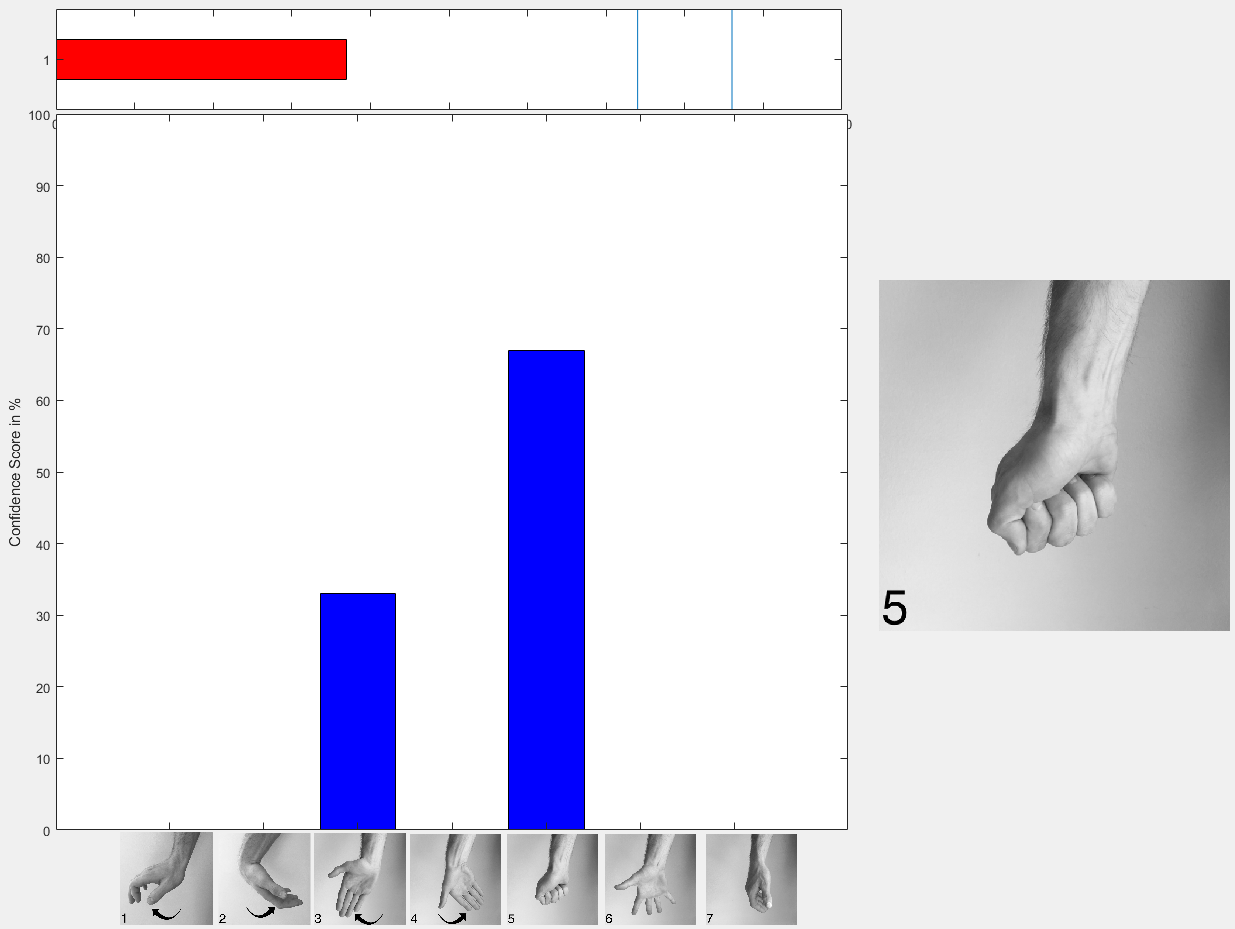
\includegraphics[width=.8\textwidth]{figures/xBackground/usertraintestGUI}  
	\caption{Illustration of the user training interface showing the bar plot indicating the confidence level of movement recognition and horizontal bar plot indicating contraction level. The picture on the right side of the bar plot indicates which movement needs to be performed.}
	\label{fig:usertraintestGUI} 
\end{figure}

\textbf{User Training} \\ %control group
The purpose of user training is for the subject to train the movements used in the performance test. During the user training the subject will train one movement at a time at different contraction levels. When training a movement, visual feedback in form of which movement the control system recognizes, is shown in a bar plot. In addition, the level of contraction is shown in a horizontal bar above the other bar plot. When performing the instructed movement at the instructed level of contraction the horizontal bar plot will appear green; if it is outside the instructed level or the control system does not recognize the performed movement, it appears red. The aim for the subject is to reach and withhold the instructed contraction level for the instructed movement while the control system recognizes it. When the subject withholds the contraction level inside the instructed contraction level for 1 seconds while the control system recognizes it the colour of the horizontal bar will appear blue. This indicates that the subject is performing well. After it has appeared blue, the subject must return to rest and perform the movement again and try to reach the instructed contraction level while the recognition of the control system matches the performed movement. An additional aim for the subject is to make the horizontal bar plot appear blue as many times as possible. The chronology of this procedure is as follows:

\begin{enumerate}
	\item Perform instructed movement at 75-85 \% contraction level for 30 seconds followed by 10 seconds rest.
	\item Perform step 1 for the remaining movements.
	\item Repeat step 1-2 at 55-65 \% contraction level.
	\item Repeat step 1-6 at 35-45 \% contraction level.
	\item Repeat step 1-6 at 15-25 \% contraction level.
\end{enumerate} 

An illustration of the interface used for user training is shown in \figref{fig:usertraincontrolGUI}.

\begin{figure}[H]                 
	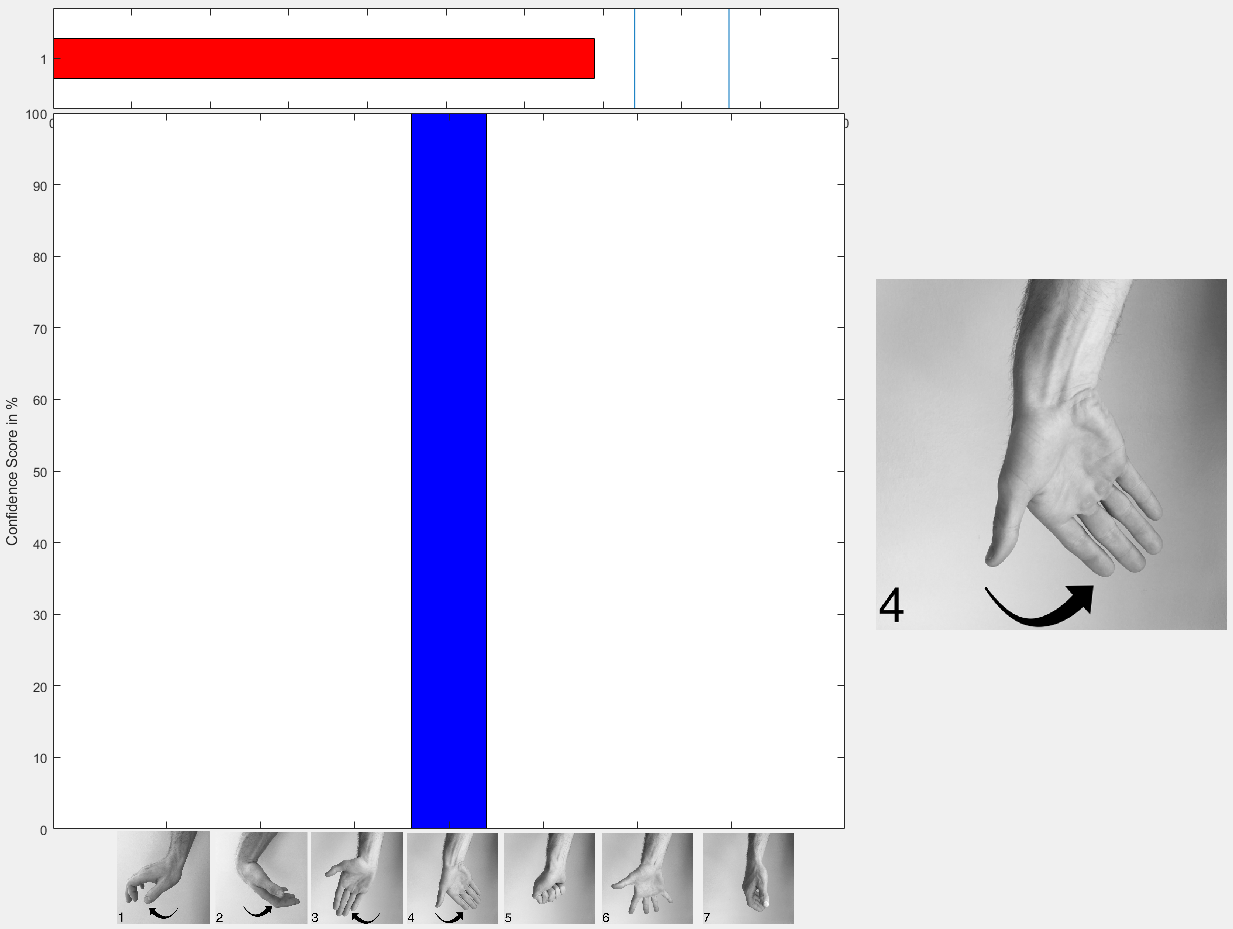
\includegraphics[width=.8\textwidth]{figures/xBackground/usertraincontrolGUI}  
	\caption{Illustration of the user training interface showing the bar plot indicating which movement is being recognized and the horizontal bar plot indicating contraction level. The picture on the right side of the bar plot indicates which movement needs to be performed.}
	\label{fig:usertraincontrolGUI} 
\end{figure}

\textbf{Performance test} \\
The purpose of the performance test is to assess the subject's ability to control a prosthesis. Instead of doing a test with a real prosthesis a virtual alternative has been developed for this experiment. The prosthesis is represented as a red circular cursor with a black dot inside in a Cartesian coordinate system, which the subject can move as well as expand and shrink in size by performing the trained movements. The following bullets describe which movement corresponds to which action in the coordinate system:

\begin{itemize}
	\item Extension moves the cursor right.
	\item Flexion moves the cursor left.
	\item Radial deviation moves the cursor up.
	\item Ulnar deviation moves the cursor down.
	\item Closed hand shrinks the cursor.
	\item Opened hand expands the cursor.
	\item Rest keeps the cursor still.
\end{itemize}

 The performance test consists of a target reaching test, where the subject must reach 16 targets of different sizes and locations. A target consists of a circle with a smaller circle inside. Only one target will be visible at a time. For the subject to reach a target and make a new appear, the subject must center the black dot of the cursor in the small circle of the target and expand/shrink the cursor to fit the size of the outer circle of the target. The cursor will appear green, when located at the correct position. The subject must dwell the cursor in a target for 1 seconds for it to be reached. When the cursor has dwelled for 1 second, it will appear blue for 1 second to indicate that the target has been reached. If a target is not reached within 15 seconds a new target will appear. When a new target appears the cursor will reset its position the origin. The aim for the subject is to reach as many target as possible as quickly as possible. The subject is only able to perform one movement at a time, as trained in the user training. Thus, no simultaneously performed movements will be recognized by the control system. %The subject will perform the test two times. In the second test the subject will need to perform smaller increases in contraction force to make the cursor move faster, compared to the first test. 
 The chronology of this procedure is as follows:

\begin{enumerate}
	\item Use 2 minutes to get acquainted with the test. 
	\item Reach the visible target.
	%\item Repeat step 1 until all targets have been shown.
	%\item Repeat step 1-3
\end{enumerate}

An illustration of the interface used for the performance test is shown in \figref{fig:perftestGUI}.

\begin{figure}[H]                 
	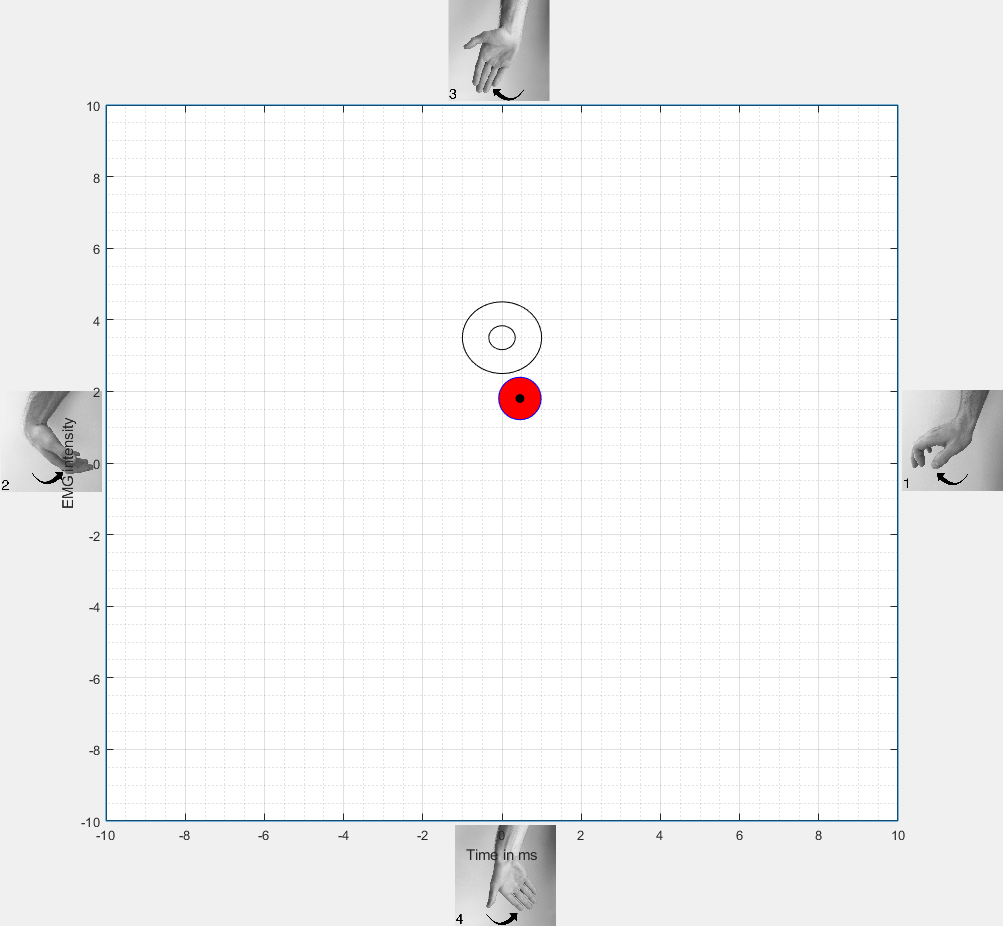
\includegraphics[width=.8\textwidth]{figures/xBackground/perftestGUI}  
	\caption{Illustration of the performance test interface showing a target and the cursor representing the prosthesis output. The pictures on the axes indicate which movement must be performed to move the cursor in a certain direction.}
	\label{fig:perftestGUI} 
\end{figure}

\newpage
\textbf{\Large Movements used in the experiment}

\begin{figure}[H]                 
	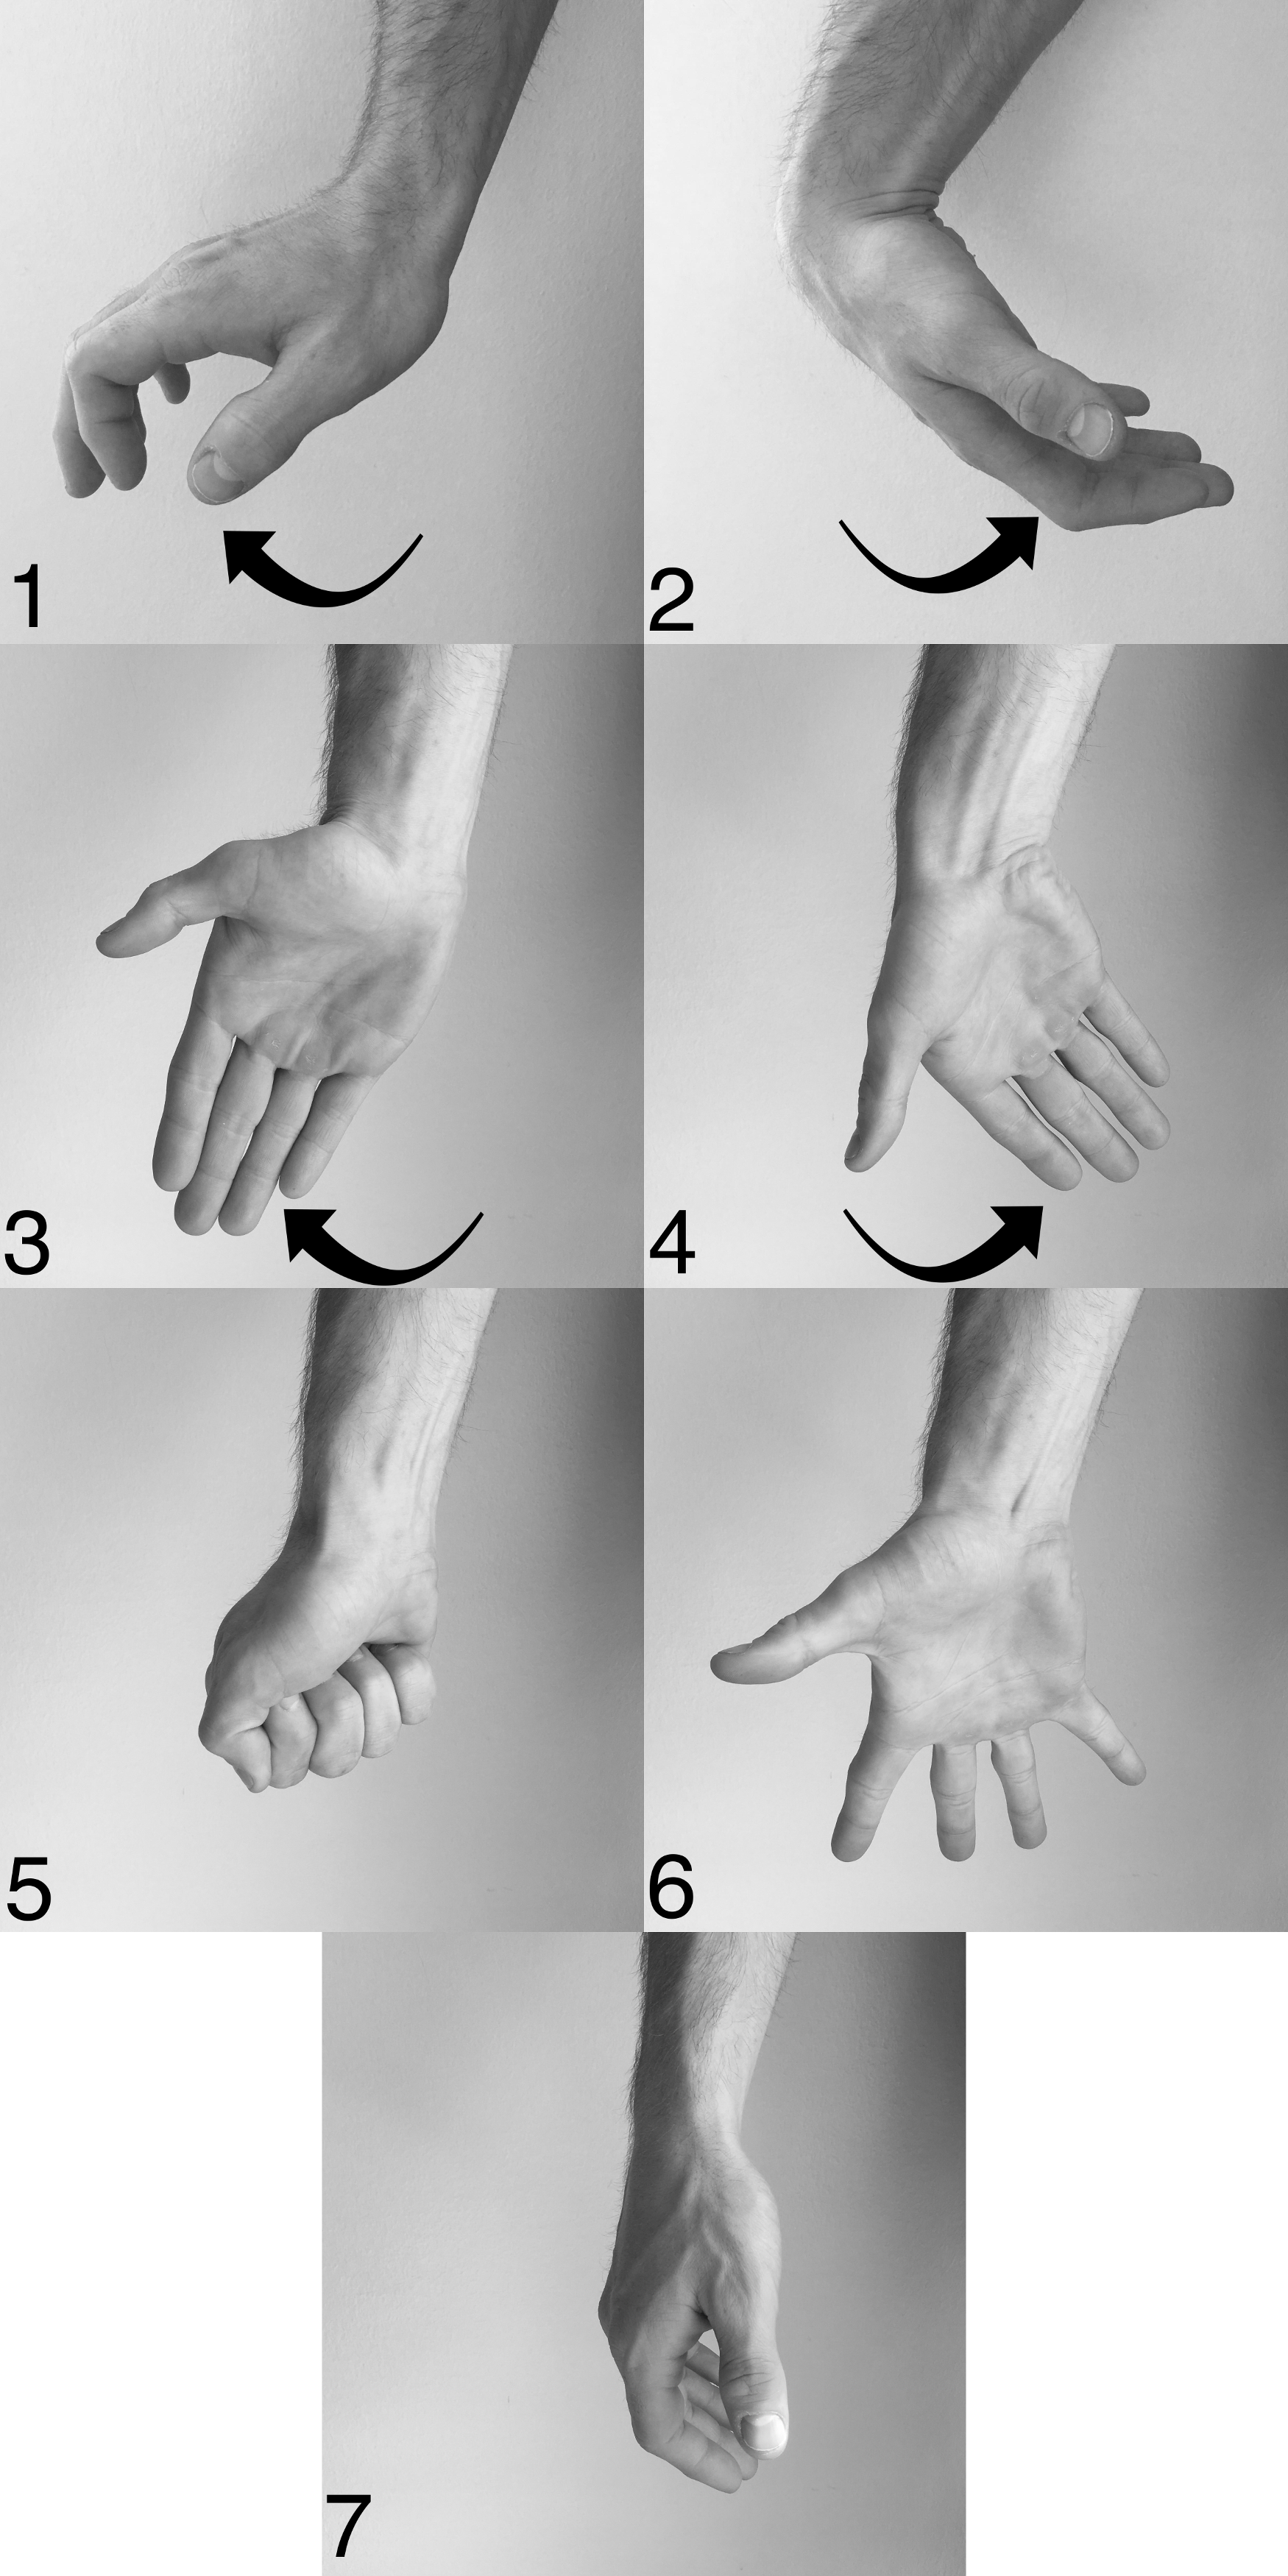
\includegraphics[width=.6\textwidth]{figures/handGestures/BW/allHandMovementsVerticalBW}  
	\caption{Illustration of the movements used in the experiment. 1: extension, 2: flexion, 3: radial deviation, 4: ulnar deviation, 5: closed hand, 6: opened hand and 7: rest.}
	\label{fig:experiment_movements} 
\end{figure}

\newpage
\textbf{\Large Experiment setup}

\begin{figure}[H]                 
	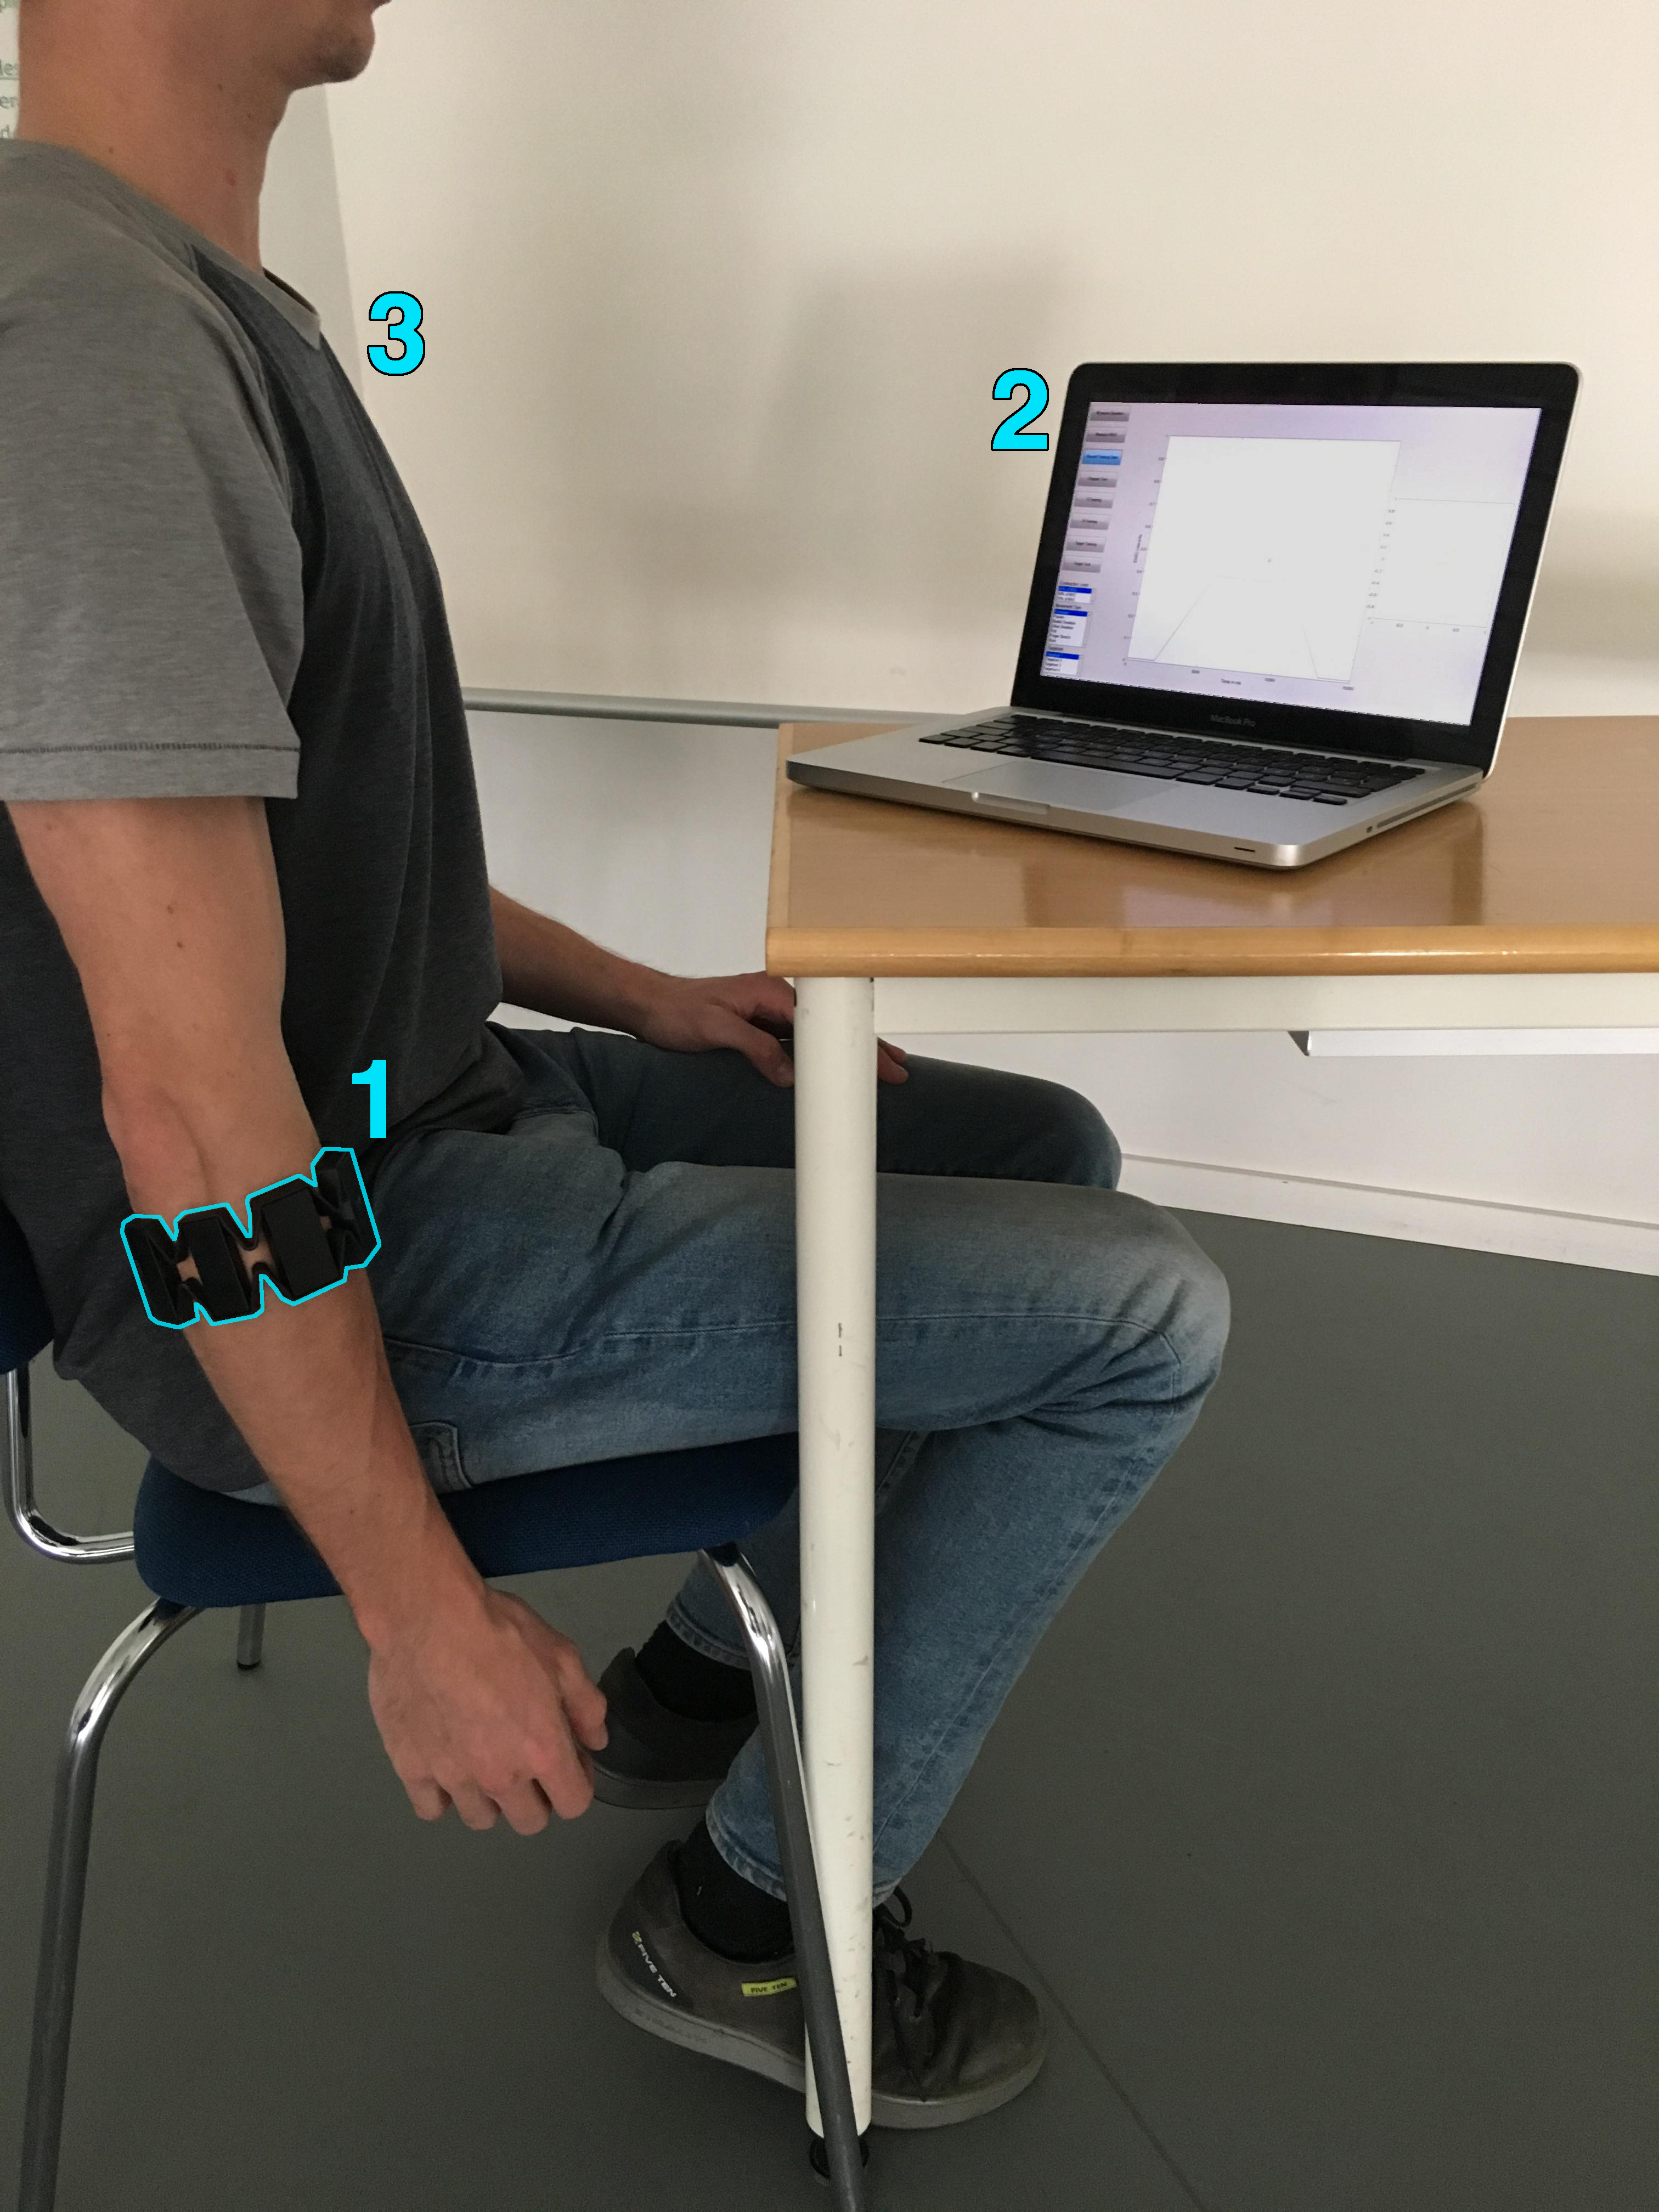
\includegraphics[width=.8\textwidth]{figures/pMethods/experimentSetup}  
	\caption{Illustration of the experimental setup; 1: MYB, 2: computer with interface and 3: subject. The subject is seated facing the computer screen with the arm wearing the MYB hanging relaxed down the side of the torso.}
	\label{fig:experiment_setup} 
\end{figure}

%Session 1) Data acquisition, user training and performance test and 2) new training data acquisition and performance test. During the training data acquisition EMG data will be recorded from the subject with an EMG-electrode armband (Myo armband from Thalmic Labs) when performing four different wrist movements(flexion, extension, radial deviation and ulnar deviation) as illustrated in \figref{FIGURE}. The data is subsequently used to fit a classification model used in the myoelectric control scheme for the following user training and performance test. Before the performance test the user is given a training period to get familiar with wrist movements used in the performance test. During the performance test the subject will perform a target-reaching task in a cartesian coordinate system of reaching a number of targets using the trained movements by controlling a cursor representing the EMG. Each axis represent one of the four wrist movements, as seen in figure \figref{FIGURE2}, and the open/close hand movements expands/contracts the size of the cursor. The aim for the subject is to reach as many targets as quickly as possible. The subject will perform the target-reaching task twice - one in each session. The subjects are divided into two groups: a test group and a control group. As the study is single-blinded the subject will not be informed which group he/she belongs to.
%
%Chronology of session 1):
%\begin{enumerate}
%	\item Apply MYB on dominant forearm at the thickest part.
%	\item Synchronize MYB by performing wrist extension until three distinct vibrations are felt.
%	\item Perform 15 seconds of maximum voluntary contraction (MVC) of instructed movement. Following the MVC the subject will be given a 30 resting period to avoid fatigue.
%	\item Perform 15 seconds contractions of respectively 20\%, 40\% and 60\% of MVC. During these contractions the subject will control a green marker representing the EMG signal and try to follow a trapezoidal trajectory a precise as possible. The trapezoidal trajectory consists of two five second transition phases and one five second plateau phase as illustrated in figure \figref{FIGURE3}. Between each trial the subject will be given a 15 seconds resting period to avoid muscle fatigue.
%	\item Repeat step 3-4 until training data from all four wrist movements has been recorded.
%	\item The subject will train the seven movements. Each movement will be performed 10 times, where each single movement consists of a five second movement with increased intensity. To improve the precision of movements the subject will receive visual feedback consisting of the probability the movement to belong to based on the classifier. The ideal probability during the training is a 100\% probability of belonging to the trained movement and a 0\% probability of belonging to the remaining movements. 
%	\item The subject will perform a target-reaching task. The subject will control an cursor  in a cartesian coordinate system representing the features extracted from the EMG data, where the length represent the intensity and direction depicts the movement performed. To reach a target the subject must dwell the head of the arrow within the target for 0.5 seconds. If this is achieved the target will disappear. The target will similarly disappear if the subject fails to achieve this within 15 seconds. When an outer target disappears a target centred in origo appears and the subject must reach this before a new outer target appears. This procedure is continued until no more targets are shown. After finishing the performance test the subject will be given a 2 minutes resting period.
%\end{enumerate}
%
%
%Chronology of session 2):
%\begin{enumerate}
%	 \item Perform step 3-5 from session 1.
%	 \item Perform step 7 from session 1. 
%\end{enumerate}
% 







